%%%%%%%%%%%%%%%%%%%%%%%%%%%%%%%%%%%%%%%%%%%%%%%%%%%%%%%%%%%%%%%%%%%%%%%%
% Escuela Politécnica Superior de la Universidad de Alicante
% Realizado por: Jose Manuel Requena Plens
% Contacto: info@jmrplens.com / Telegram:@jmrplens
%%%%%%%%%%%%%%%%%%%%%%%%%%%%%%%%%%%%%%%%%%%%%%%%%%%%%%%%%%%%%%%%%%%%%%%%

\definecolor{mycolor1}{rgb}{1.00000,0.00000,1.00000}%
%
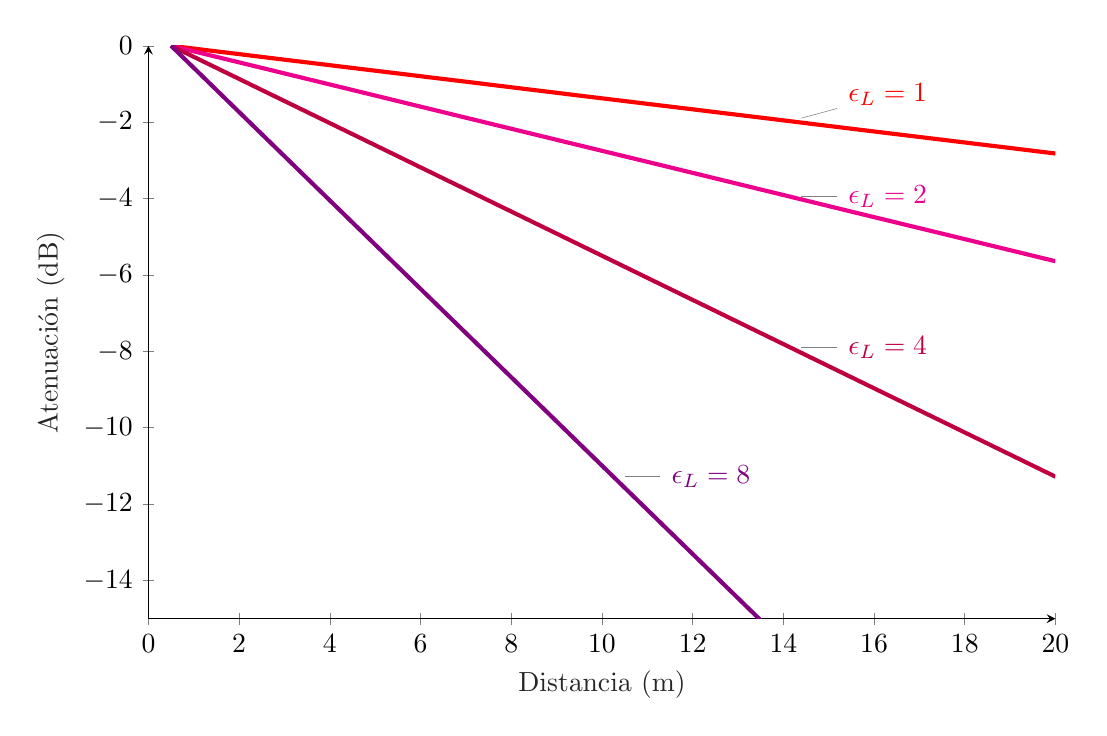
\begin{tikzpicture}

\begin{axis}[%
width=0.95\textwidth,
height=0.6\textwidth,
at={(0\textwidth,0\textwidth)},
scale only axis,
xmin=0,
xmax=20,
xlabel style={font=\color{white!15!black}},
xlabel={Distancia (m)},
ymin=-15,
ymax=0,
axis y line=left,
axis x line=bottom,
ylabel style={font=\color{white!15!black}},
ylabel={Atenuación (dB)},
axis background/.style={fill=white},
legend style={legend cell align=left, align=left, draw=white!15!black}
]



\addplot [color=red, line width=1.5pt,domain=0.5:20, samples=10]
{10*ln(1.0337e+12*(3.5407e-04*e^(-(13.82*(x/343+0.05)*1/1.2098))))/ln(10) - 10*ln(1.0337e+12*(3.5407e-04*e^(-(13.82*(0.5/343+0.05)*1/1.2098))))/ln(10)} node [pos=0.7,pin=5:{$\epsilon_L=1$}] {};

\addplot [color=magenta, line width=1.5pt,domain=0.5:20, samples=10]
{10*ln(1.0337e+12*(3.5407e-04*e^(-(13.82*(x/343+0.05)*2/1.2098))))/ln(10) - 10*ln(1.0337e+12*(3.5407e-04*e^(-(13.82*(0.5/343+0.05)*2/1.2098))))/ln(10)} node [pos=0.7,pin=0:{$\epsilon_L=2$}] {};

\addplot [color=purple, line width=1.5pt,domain=0.5:20, samples=10]
{10*ln(1.0337e+12*(3.5407e-04*e^(-(13.82*(x/343+0.05)*4/1.2098))))/ln(10) - 10*ln(1.0337e+12*(3.5407e-04*e^(-(13.82*(0.5/343+0.05)*4/1.2098))))/ln(10)} node [pos=0.7,pin=0:{$\epsilon_L=4$}] {};

\addplot [color=violet, line width=1.5pt,domain=0.5:20, samples=10]
{10*ln(1.0337e+12*(3.5407e-04*e^(-(13.82*(x/343+0.05)*8/1.2098))))/ln(10) - 10*ln(1.0337e+12*(3.5407e-04*e^(-(13.82*(0.5/343+0.05)*8/1.2098))))/ln(10)} node [pos=0.5,pin=0:{$\epsilon_L=8$}] {};

\end{axis}
\end{tikzpicture}%